\newpage
\section{Experiments}\label{sec:exp}
Our experiments are based on the three ILP techniques discussed in the previous sections. 
During the implementation, value was placed on the best possible comparability. For example, all three realisations use the same labyrinths and logically identical or similar predicates.
However, since the implementations of the three techniques were run on different computers, the timing results are only comparable to a limited extent.\\
Table~\ref{tab:prf_cmp} offers an overview of the timings of the main tasks presented in Section~\ref{sec:impl}.
{\rowcolors{2}{gray!50!}{}
\begin{center}
    \begin{table}[h]
    \centering
    \begin{tabular}{ |l|c|c|c| } 
        \hline
        Task & \textbf{HYPER} & \textbf{Metagol} & \textbf{ILASP} \\ \hline
        \texttt{adjacent/2} & 175.884 & 0.056 & 4.767 \\ 
        \texttt{move/2} & 0.063 & 0.047 & 5.343 \\ 
        \texttt{move/2} (\(7*7\) grid) & 0.0716 & 0.054 & 5.432 \\
        \texttt{move/2} (\(9*9\) grid) & 0.0718 & 0.023 & 5.381 \\
        \texttt{reach/3} & 1.577 & 0.027 & NA \\ 
        \texttt{move/2} and \texttt{reach/3} & 7.077 & 0.848 & NA \\ 
        \hline
    \end{tabular}
    \caption{\label{tab:prf_cmp}Time comparison between the different systems for the main tasks (seconds)}
\end{table}
\end{center}
}
The maze dimension do not seem to have an impact on the learning process (as for ILASP this is described
in another context at Section~\ref{sec:ilasp} and for Hyper in section ~\ref{sec:hyper}).\\
Table ~\ref{tab:prf_cmp} also shows the similar behavior between HYPER and Metagol in terms of the \emph{combined
learning} of predicates \texttt{move/2} and \texttt{reach/3}. Both the implementations seem to
perform better in learning complex predicates when the tasks are split into smaller ones.
Comparing the timings overall, it can be noticed, that Metagol performs much better than the other
two systems. Given the similar approaches of HYPER and Metagol, one could expect them
to also have similar performances. While HYPER uses a more general approach, Metagol owes its efficiency to metarules and the way they shape the language bias. This, though, does not come
for free, since defining good metarules requires a very accurate initial idea of what the final solution should be like.\\

The time performances are also measured in order to analyze the behavior of the systems with different sets of positive examples.
For this experiment, we measured the performances of the implementations to learn the predicate \texttt{move/2} (\emph{learning to walk}) on more redundant examples than are actually needed.
The results of these experiment can be seen in Table~\ref{tab:ex_cmp}.
{\rowcolors{2}{gray!50!}{}
\begin{center}
    \begin{table}[h]
    \centering
    \begin{tabular}{ |l|c|c|c| } 
        \hline
        \(|E^+|\) & \textbf{HYPER} & \textbf{Metagol} & \textbf{ILASP} \\ \hline
        8 & 0.067 & 0.029 & 5.31 \\ 
        16 & 0.065 & 0.028 & 5.43 \\
        24 & 0.065 & 0.033 & 5.53 \\  
        \hline
    \end{tabular}
    \caption{\label{tab:ex_cmp}Time comparison with increasing examples (seconds)}
\end{table}
\end{center}
}
The timing measurements show, that the different quantities of positive examples do not impact the performances. However, this may not be true for way larger
quantities. 
For example, Metagol would have to prove all of these examples one after the other, and although this would be a trivial task, very large numbers of positive examples could have run-time effects.

\subsection{Learning \texttt{reach/3} with \emph{tail recursion}}
Being \emph{"solving the Maze problem"} part of the title and one of the main goals of this project, we were
quite surprised that the \texttt{reach/3} predicate learned in our implementations was not able to find a path
in our Maze (Figure~\ref{fig:our}).\\
By studying the trace when querying Prolog with \texttt{reach((1,1), (2,5), L)},
we noticed that the search of the path would get stuck into a loop, going back and forth from cells \texttt{(5,2)} and
\texttt{(5,3)}. The reason of this behavior is related to the (partly) declarative nature of Prolog. The \texttt{reach/3}
predicate defined as in Listing~\ref{lst:res_rfsm} falls into a loop because, when getting at cell \texttt{(5,2)},
the predicate \texttt{reach\_2/2} is unified with the head of the first rule found in the program. Since there is
no \texttt{B} such that \texttt{inc\_x((5,2),B)}, Metagol will go for \texttt{dec\_y((5,2), B)}. This unification
will not work either since there is no \texttt{B} such that \texttt{dec\_y((5,2), B)} (\texttt{(5,1)} is an obstacle). At
last the unification is done with the rule at Line 5, with the body consisting to \texttt{inc\_y((5,2), B)} and hence moving
to cell \texttt{(5,3)}.\\
Now again, there is no \texttt{B} such that \texttt{inc\_x((5,3), B)}, so Metagol will unify the
\texttt{reach\_2/2} predicate with the head of the rule at Line 4, going for \texttt{dec\_y((5,3), B)} and, hence,
going back onto cell \texttt{(5,3)}.\\

In order to solve this issue we were able to \emph{"manually"} define a procedure for \texttt{reach/3} as shown in Listing~\ref{lst:r_tr}

\begin{figure}
    \centering
    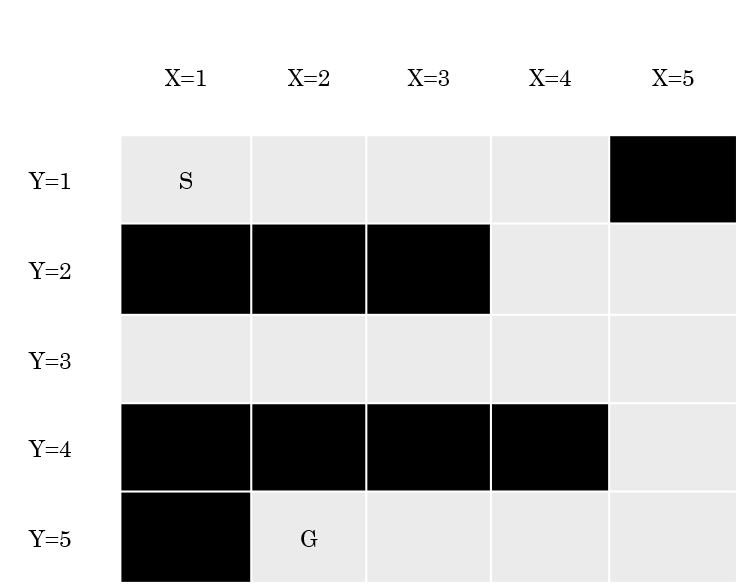
\includegraphics[scale=0.7]{img/ourMaze.png}
    \caption{The analyzed Maze}\label{fig:our}
\end{figure}

\begin{lstlisting}[label={lst:r_tr}, language=Prolog, caption=\texttt{reach/3} with tail recursion, belowcaptionskip=1cm]
reach(A,B,L) :- reach_1(A,B,[A],L).
reach_1(A,A,L,L).
reach_1(A,B,Acc,L) :-
    move(A,C),
    non_member(C,Acc),
    reach_1(C,B,[C|Acc],L). 
\end{lstlisting}
This procedure resembles the techniques for a loop preventing Depth-First Search. The idea behind this procedure is to store
the already visited cells into an accumulator (\texttt{Acc}) and, at each step, check whether a new encountered cell has already
been visited before.\\
Unfortunately, we were not able to learn this procedure through any of the mentioned ILP techniques.
\newpage